
%----------------------------------------------------------------------------------------
%	PACKAGES AND DOCUMENT CONFIGURATIONS
%----------------------------------------------------------------------------------------

\documentclass{article}

%\usepackage{mhchem} % Package for chemical equation typesetting
%\usepackage{siunitx} % Provides the \SI{}{} command for typesetting SI units
\usepackage[T1]{fontenc}
\usepackage[utf8]{inputenc}
%
\usepackage[swedish]{babel}
\usepackage{graphicx} % Required for the inclusion of images
\usepackage{float}
\usepackage{caption}
\usepackage{subcaption}

%Matte
\usepackage{amsmath}
\usepackage[makeroom]{cancel}
\usepackage{gensymb} % \degree

\setlength\parindent{0pt} % Removes all indentation from paragraphs
%\renewcommand{\labelenumi}{\alph{enumi}.} % Make numbering in the enumerate environment by letter rather than number (e.g. section 6)
%\usepackage{times} % Uncomment to use the Times New Roman font

%%% För kod!
\usepackage{listingsutf8}
\usepackage{color}
\definecolor{dkgreen}{rgb}{0,0.6,0}
\definecolor{gray}{rgb}{0.5,0.5,0.5}
\definecolor{mauve}{rgb}{0.58,0,0.82}
\lstset{frame=tb,
  language=Matlab,
  aboveskip=3mm,
  belowskip=3mm,
  showstringspaces=false,
  columns=flexible,
  basicstyle={\small\ttfamily},
  numbers=none,
  numberstyle=\tiny\color{gray},
  keywordstyle=\color{blue},
  commentstyle=\color{dkgreen},
  stringstyle=\color{mauve},
  breaklines=true,
  breakatwhitespace=true
  tabsize=3
  extendedchars=\true,
  inputencoding=utf8/latin1
}
%%%% slut kod



%----------------------------------------------------------------------------------------
%	DOCUMENT INFORMATION
%----------------------------------------------------------------------------------------

\title{Elteknik - inlämning 1} % Title

\author{
	\begin{tabular}{l r}
    Marcus Olsson \\
    %number & number & number% Author name
    \\
    \end{tabular}
    }

\date{\today} % Date for the report

\begin{document}

\maketitle % Insert the title, author and date
\tableofcontents
\clearpage
%----------------------------------------------------------------------------------------
%	SECTION 1
%----------------------------------------------------------------------------------------
\section{Intro}
Beräkningar är gjorda i MATLAB och koden finns i Appendix.

%----------------------------------------------------------------------------------------
%	SECTION 2
%----------------------------- -
\section{A - Elnät}
Ett litet elnät planeras med följande laster vid 400V

\begin{enumerate}
	\item Flerfamiljehus – den beräknade toppeffekten är 250 kW, $cos\varphi = 0,98$.
	\item Förskola och andra samlingslokaler – effektbehovet max 100 kVA, $cos\varphi = 0,95$
	\item En symmetrisk trefas, Y – kopplad asynkronmotor med märkspänning 400 V,
märkström 200 A och $cos\varphi = 0,8$. Parallellt med motorn är ett kondensatorbatteri
inkopplat som är märkt 90 kVAr.
\end{enumerate}

\subsection{a}
Här ska fasströmmen som respektive last drar beräknas.
Ett visardiagram skall ritas för varje ström samt den totala strömmen, fas a används som referens.
Ekvikalenta impedanser skall också beräknas.
Här antas symmetriska laster.

  \subsubsection{Fasströmmar}
  Effekten i flerfamiljehuset är 250kW, eftersom enheten är watt är det aktiv effekt som är beräknat.
  Jag använder [\ref{P},\ref{I}] för att beräkna strömmen $I_1$ där $U=400\angle{0\degree}$
  Detta ger mig $I_1=368\angle{-11.5\degree}=361-j73.3 A$

  \begin{equation}
    \underline{I} = I\angle{-\varphi}
    \label{I}
  \end{equation}

  \begin{equation}
    P=\sqrt3UIcos\varphi
    \label{P}
  \end{equation}

  Effekten för förskolan är skriven i Voltampere, detta betyder att det är skenbar effekt som är beräknat.
  Då använder jag [\ref{S},\ref{I}] och löser ut $I_2$ för att få fram att $I_2=(I_2^*)^*=144\angle{-18.2\degree}=137-j45 A$

  \begin{equation}
    S=\sqrt3UI^*=P+jQ
    \label{S}
  \end{equation}

  Motorn är parallellkopplad med ett kondensatorbatteri för att faskompenseras och därmed dra en lägre total reaktiv effekt.
  Här används [\ref{Q},\ref{P},\ref{S}] för att få fram aktiv och reaktiv effekt för motorn.
  Effekterna kan sedan summeras eftersom de är parallellkopplade för att få fram den totala skenbara effekten.
  Efter detta kan jag göra precis som i förra upgiften för att lösa ut $I_3=160\angle{3.54\degree}=160+j9.9 A$

  \begin{equation}
    Q=\sqrt3UIsin\varphi
    \label{Q}
  \end{equation}

  När dessa är beräknade så kan man enkelt räkna ut den totala strömmen genom att summera de enskilda komplexa strömmarna.
  Detta ger $I_{tot}=658-j108 = 667\angle{-9.3\degree} A$

  \subsubsection{Impedanser}
  De ekvivalenta impedanserna fås ur Ohms lag [\ref{ohms}], dessa blir följande:
  \begin{equation}
    Z=\frac{U_f}{I_f}=\frac{U}{\sqrt{3} I_f}
    \label{ohms}
  \end{equation}

  \begin{tabular}{l}
    $z_1=0.61 + j0.12$\\
    $z_2=1.52 + j0.50$\\
    $z_3=1.44 - j0.09$\\
    $z_{tot}=0.34 + j0.056$\\
  \end{tabular}

  \subsubsection{Visardiagram}
  Här är visardiagram för strömmarna $I_1 - I_{tot}$ för första fasen, detta eftersom det är symmetriska laster.


  \begin{figure}[H]
  \begin{center}
  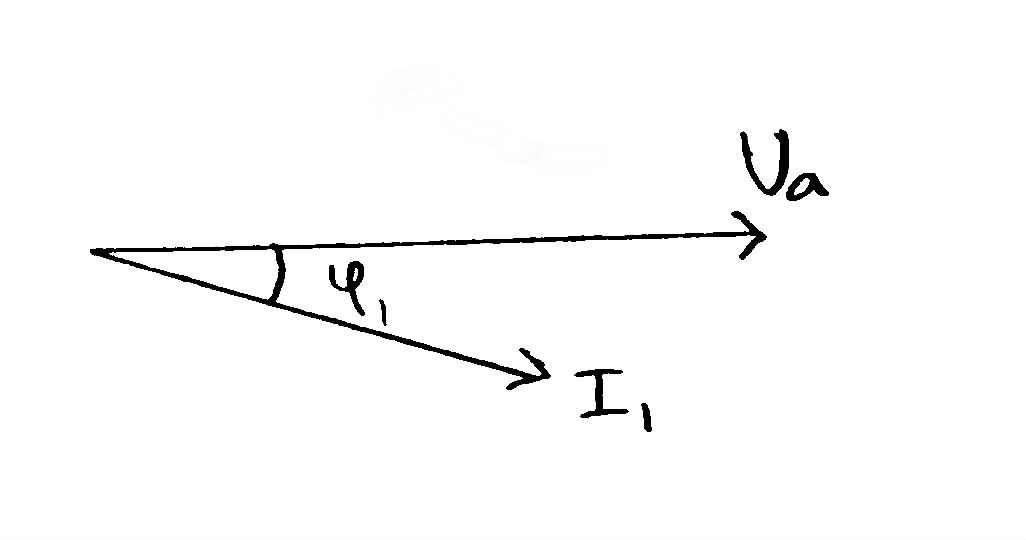
\includegraphics[width=0.7\textwidth]{img/I1.jpg} % Include the image placeholder.png
  \caption{Strömmen $I_1$}
  \end{center}
  \end{figure}

  \begin{figure}[H]
  \begin{center}
  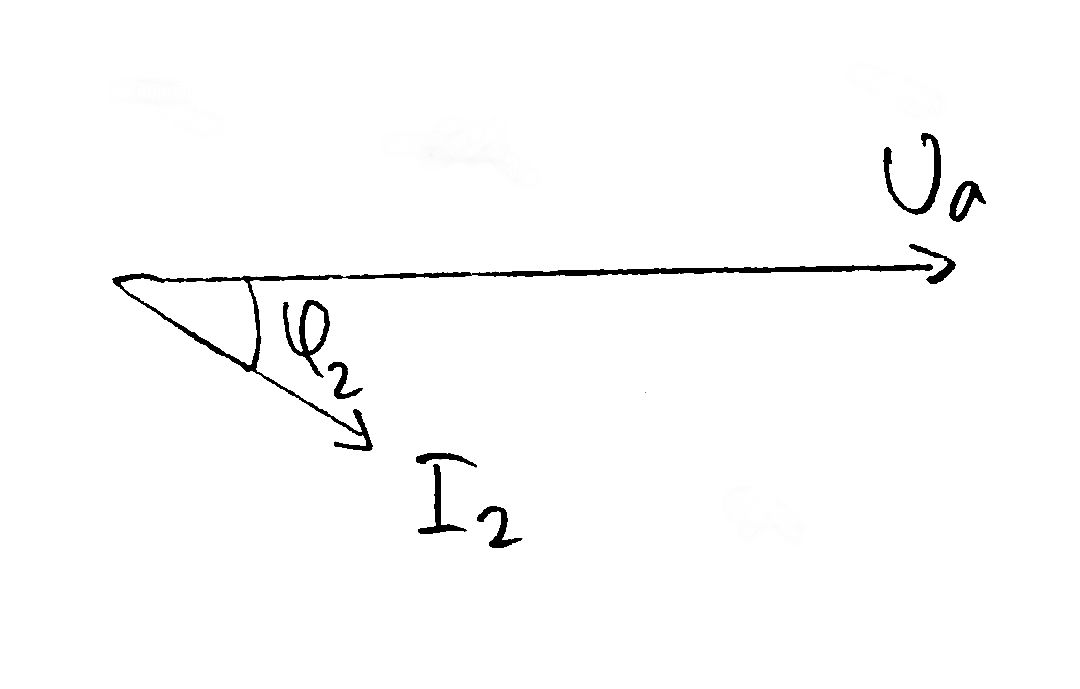
\includegraphics[width=0.7\textwidth]{img/I2.jpg} % Include the image placeholder.png
  \caption{Strömmen $I_2$}
  \end{center}
  \end{figure}

  \begin{figure}[H]
  \begin{center}
  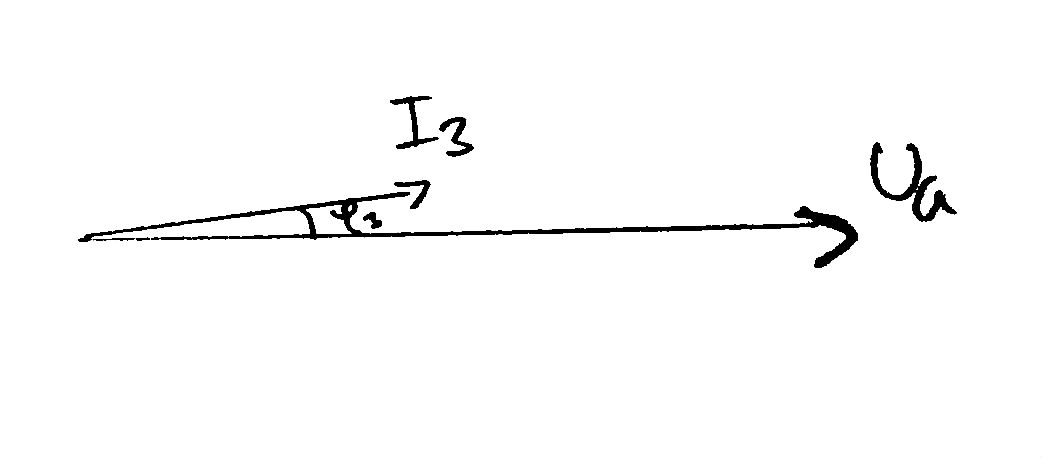
\includegraphics[width=0.7\textwidth]{img/I3.jpg} % Include the image placeholder.png
  \caption{Strömmen $I_3$}
  \end{center}
  \end{figure}

  \begin{figure}[H]
  \begin{center}
  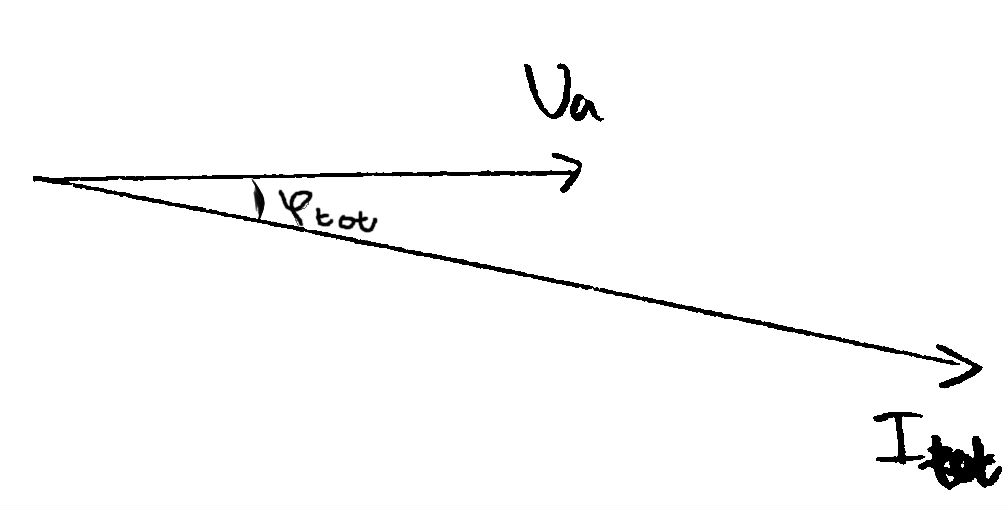
\includegraphics[width=0.7\textwidth]{img/Itot.jpg} % Include the image placeholder.png
  \caption{Totala strömmen}
  \end{center}
  \end{figure}

\subsection{b}
  Här ska den skenbara effekten beräknas, för alla laster inkopplade och var och en för sig.
  Ekvation [\ref{S}] används för de olika lasterna och då fås följande resultat.
  Eftersom vinkeln för $S_{tot}$ är positiv så är den totala lasten induktiv.

  \begin{tabular}{l}
      $S_1=250 + j28.7 kVA$ \\
      $S_2=95+ j31.2 kVA$ \\
      $S_3 = 111 -  j6.86 kVA$\\
      $S_{tot}=456 + j53.1 kVA$
  \end{tabular}

\subsection{c}
Den tredje lasten är faskompenserad med ett kondensatorbatteri.
Detta gör man ofta på större motorer för att minska den reaktiva effekten i nätet.
Eftersom den reaktiva effekten för kondensatorn är större än för motorn blir nettoeffekten negativ och strömmen får en positiv vinkel.


%----------------------------------------------------------------------------------------
%	SECTION 3
% %----------------------------------------------------------------------------------------
\section{B - Osymmetrisk trefas}
  En osymmetrisk trefas är kopplad till en huvudspänning på $U_{ab}=400V$
  Fasströmmarna samt strömmen genom varje impedans skall beräknas.
  Ett visardiagram skall också ritas med $U_{ab}$ som referens.
  \\
  \\
  Jag börjar med att sätta ut referenser för strömmarna enligt Figur \ref{fig:osymm} och använder Ohms lag [\ref{Ohms}]\
   med spänningarna $U_1=400\angle{0\degree},U_2=400\angle{-120\degree},U_3=400\angle{-240\degree}$ för att beräkna strömmarna över varje last.
  Efter detta använder jag KCL enligt nedan för att få fram fasströmmarna.


  \begin{tabular}{| l}
    $I_{ab}=4.8-j6.4=8\angle{-53.1\degree}$\\
    $I_{bc}=-2-j3.46=4\angle{-120\degree}$\\
    $I_{ac}=-14.71+j6.29=16\angle{156.9\degree}$\\
    \\
    $I_a=I_{ab}+I_{ac}=-9.9-j0.11=9.9\angle{-179.3\degree}$\\
    $I_b=I_{bc}-I_{ab}=-6.8+j2.94=7.41\angle{156.6\degree}$\\
    $I_c=-(I_{bc}+I_{ac})=16.7-j2.82=16.95\angle{-9.58\degree}$\\
  \end{tabular}


  \begin{figure}[H]
  \begin{center}
  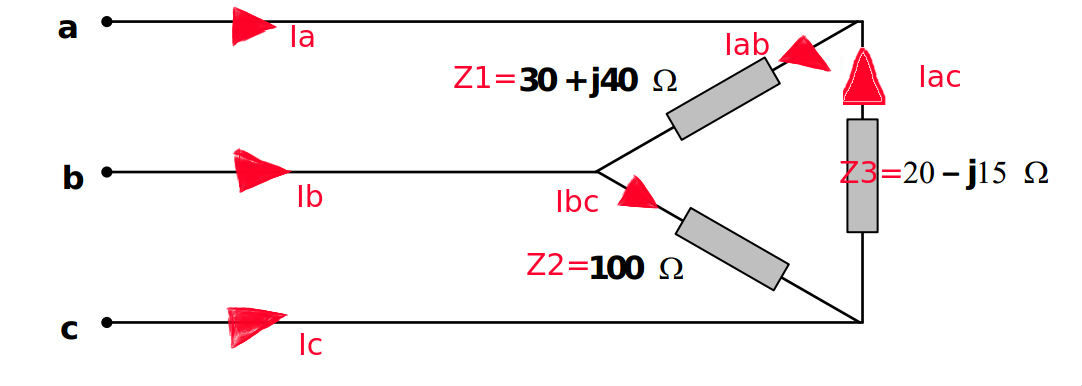
\includegraphics[width=1\textwidth]{img/osymmetrisk-last1.jpg} % Include the image placeholder.png
  \caption{Osymmetrisk last med strömreferenser inritade}
  \label{fig:osymm}
  \end{center}
  \end{figure}


%----------------------------------------------------------------------------------------
%	SECTION 4
%----------------------------------------------------------------------------------------
\section{C}
\subsection{a}
lorem
\subsection{b}
ipsum
%----------------------------------------------------------------------------------------
%	SECTION 5
%----------------------------------------------------------------------------------------
\section{D - Transformator}
Det gäller att dimensionera en 50 Hz enfastransformator med märkeffekten Sn, primärspänningen
U1n och sekundärspänningen U2n med användning av ett givet plåtsnitt. Plåtsnittets dimensioner
är angivna i figur \ref{fig:trafo}.
$Sn = 1160 VA, U1n = 220 V,U2n = 110 V$


 \begin{figure}[H]
 \begin{center}
 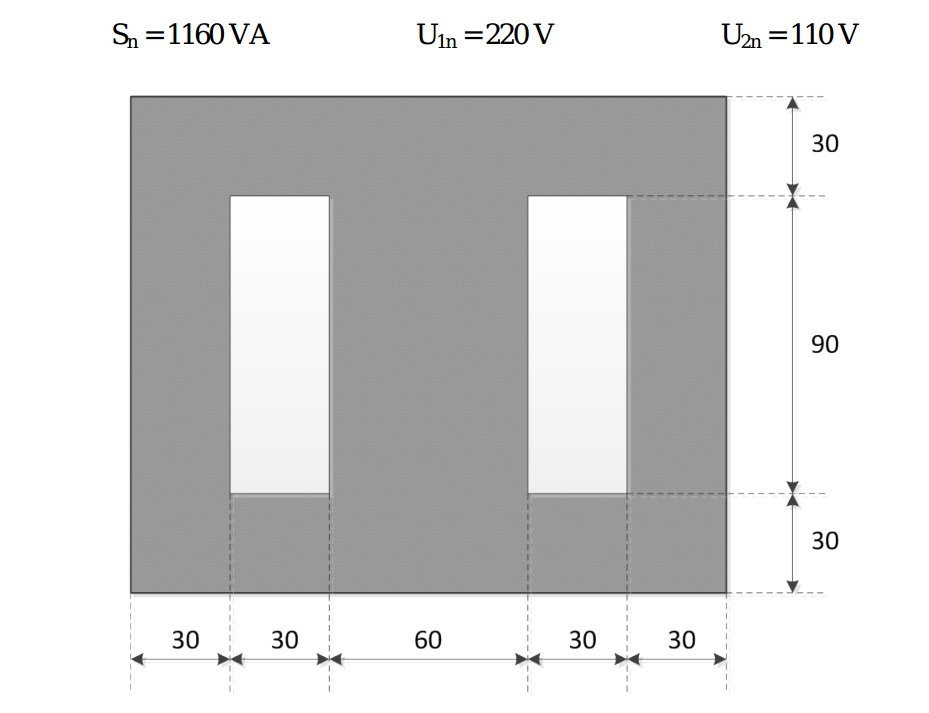
\includegraphics[width=1\textwidth]{img/transformatorplat.png} % Include the image placeholder.png
 \caption{Transformatorplåtens dimensioner}
 \label{fig:trafo}
 \end{center}
 \end{figure}

\subsection{a}
Märkströmmarna beräknas med [\ref{markstrom}] och blir:
\begin{tabular}{|l}
  $I_1=5.27 A$\\
  $I_2=10.55 A$\\
\end{tabular}
\\
Transformatoromsättningen blir enligt [\ref{n}] $n=2$.

\begin{equation}
  I=\frac{S}{U}
  \label{markstrom}
\end{equation}

\begin{equation}
  n=\frac{N_1}{N_2}=\frac{U_1}{U_2}
  \label{n}
\end{equation}

\subsection{b}
Lindningarna skall lindas på en plastbobbin enligt Figur \ref{ref:bobbin} den disponibla lindningsarean skall beräknas.
Den totala bredden för $b_1+b_2=30-(bobbin+isolering+distans)$ Detta ger en total lindningsbredd.
En total lindningshöjd blir då $90-2bobbin$.
Produkten av dessa ger lindningsarean $A_L=(b_1+b_2)h=1804 mm^2$

 \begin{figure}[H]
 \begin{center}
 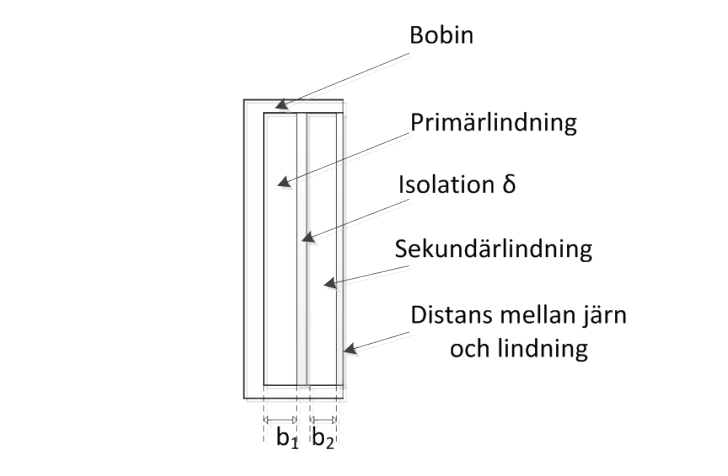
\includegraphics[width=1\textwidth]{img/bobbin.png} % Include the image placeholder.png
 \caption{Bobbin}
 \label{fig:bobbin}
 \end{center}
 \end{figure}


\subsection{c}
En fyllfaktor $k_{Cu}=[0.6 - 0.7]$ enligt [\ref{Kcu}]  finns, intervallet för $A_Cu$ skall beräknas.
Detta ger ett intervall på $A_{Cu}=[1082 - 1263] mm^2$


\begin{equation}
  k_{Cu}=\frac{A_{Cu}}{A_L}
  \label{Kcu}
\end{equation}

\subsection{d}
Ledardiameter $d_1,d_2$ och ledartvärsnitten $A_1,A_2$ skall beräknas.
Strömtätheten för primärlindningen ligger mellan $J_p=[1.5 - 1.8] A/mm^2$ och sekundärlindningen mellan $J_s=[1.9 - 2.1] A/mm^2$

Detta görs enligt [\ref{AIJ}] och ger:
\begin{tabular}{|l}
  $A_1=[ 3.52 - 2.93] mm^2$\\
  $A_2=[ 5.55 - 5.02] mm^2$\\
\end{tabular}

\begin{equation}
  A=\frac{I}{J}
  \label{AIJ}
\end{equation}

\subsection{e}
Här ska intervallet för $N_1,N_2$ beräknas.
Detta görs med [\ref{NACu}], Jag bryter ut $A_{Cu}$ och byter ut $N_1$ enligt [\ref{N1N2}] och avrundar nedåt.
Då fås:

\begin{tabular}{|l}
  $N_1=[ 172 - 232]  varv$\\
  $N_2=[ 86 - 116]  varv$\\
\end{tabular}

\begin{equation}
  N_1=2N_2
  \label{N1N2}
\end{equation}

\begin{equation}
  N_1A_1+N_2A_2=A_{Cu}
  \label{NACu}
\end{equation}


\subsection{f}
Lindningarna $N_1,N_2$ och lindningstjocklekarna $b_1,b_2$ skall väljas så att lindningen får plats i fönstret\
och så att $k_{Cu}$ är inom rätt intervall.

Jag börjar med att välja de kabeldiametrar som finns inom det intervall som beräknats i $d)$.
Dessa är $d_1=2.00 mm,d_2=2.60 mm$.
Sedan måste en isolation på $0.1 mm$ adderas till diametrarna.
Varvantalet väljs till det i mitten av intervallet, $N_1=202, N_2=101$.
Kopparareorna beräknas enligt [\ref{Acu}], den totala koppararean blir då $A_{Cu}=A_{Cu1}+A_{Cu2}$.
Då kan fyllfaktorn beräknas enligt [\ref{Kcu}] och blir $k_{Cu}= 0.58$.
Efter detta beräknas $b_1,b_2$ enligt [\ref{bn}] och blir:
\begin{tabular}{|l}
  $b_1=14.67 mm$\\
  $b_2=7.33 mm$\\
\end{tabular}


\begin{equation}
  A_{Cu}=N\pi(\frac{d+0.1}{2})^2
 \label{Acu}
 \end{equation}

\begin{equation}
  b_n=\frac{A_{Cun}}{h k_{Cu}}
  \label{bn}
\end{equation}

\subsection{g}
Den magnetsika flödestäthetens toppvärde skall beräknas och vara inom intervallet $B_{max}=[1.1 - 1.2] T$.
Plåtpaketets tjocklek skall också beräknas.
Detta skall vara något av följande $t = 62, 77, 92 mm$.
Järnets fyllfaktor är antingen $k_{Fe}=0.90$ eller $0.95$.

Transformatorformeln [\ref{trafo},\ref{Bphi}] används för att beräkna järnets area.
Enligt Figur \ref{fig:trafo} är bredden på järnkärnan $60 mm$, detta används för att få fram djupet.
Detta ger fyra alternativ mellan $[72 - 84] mm$, då väljs $d=77 mm$ och $k_{Fe}=0.95$.
Då fås $B_{max}=1.19$ vilket passar i intervallet.


\begin{equation}
  U_1=4.4 f N_1 \phi
  \label{trafo}
\end{equation}

\begin{equation}
  \phi=B_{max} A
  \label{Bphi}
\end{equation}

\subsection{h}
Följande värden skall beräknas med hjälp av tidigare värden:

\begin{itemize}
  \item Lindningarnas resistans
  \item Läckreaktans
  \item Kopparförluster vid märkdrift
  \item Tomgångsförluster
  \item Tomgångsström
\end{itemize}

\subsubsection{Resistans}
Resistansen i ledningarna bestäms med [\ref{R}] där $l$ är längden på lindningarna.
Längden på lindningarna beräknas med [\ref{L}] där bobbinen antas vara cylindrisk och medelvärdet på lindningarna används och $A$ är ledarens koppararea.
Radien är (järnkärna$+bobbin+\frac{b}{2})$ enligt figur \ref{fig:bobbin}.
Då fås $R_1=0.29 \ohm,R_2=0.078 \ohm$ men $R_k=R_1+R_2'$.
Vilket blir $R_k=R_1+R_2 (N_1/N_2)^2=0.60 \ohm$

\begin{equation}
  R=\frac{\rho l}{A}
  \label{R}
\end{equation}

\begin{equation}
  l=2 r \pi N
  \label{L}
\end{equation}

\subsubsection{Läckreaktans}
Läckreaktansen räknas enligt [\ref{Xd}] där $l_m$ är medelvarvslängen och $\delta$ är avståndet mellan lindningarna.
I detta fall blir läckreaktansen $X_k=1.01 \ohm $

\begin{equation}
  X_\sigma = \frac{2 \pi \mu_0 l_m N_1^2}{h} (\delta + \frac{b_1 + b_2}{3})
  \label{Xd}
\end{equation}

\subsubsection{Kopparförluster}
Kopparförlusterna är de förluster som sker i transformatorn på grund av resistansen i lindningarna.
Den kommer att vara $P_{Cu}=R_1 I_1^2 +R_2I_2^2=16.64 W$

\subsubsection{Tomgångsförluster}
Tomgångsförlusterna eller järnförlusterna är förlusten som beror på järnkärnans resistans.
Vi kan läsa av förlustkurvan enligt våra beräkningar för $B_max$ och får då $P_{Fe}=1.9 W/kg$.
Massan på Järnet beräknas till $M_{Fe}= 10.93 kg$ och ger oss då $P_0=20.76 W$.

% \begin{equation}
%   P_{Fe}=\frac{U_1^2}{R_{Fe}}
%   \label{Pfe}
% \end{equation}

\subsubsection{Tomgångsström}
$I_{02}$...???

\subsection{i}
Jämför värdena $R_k,X_k,P_0,I_0$ med praktiska värden från ett kortsutningsprov och ett tomgångsprov.

\begin{tabular}{l l l}
  $I_k = 5,30 A$ & $U_k = 5,5 V $&$ P_k = 25 W$\\
  $U_0 = 110 V $&$ I_0 = 0,43 A $&$ P_0 = 17 W$\\
\end{tabular}

Då man jämför kortslutningsvärdena ($R_k,X_k$) så använder man [\ref{Zk},\ref{phik},\ref{Rk},\ref{Xk}] och ser att\
$R_k= 0.89$ vilket är lite större än mitt beräknade.
Detta kan kanske bero på att det är olika antal varv och kopparareor, vilket påverkar resistansen.
$X_k= 0.53$ vilket är mindre än det beräknade, detta kan bero på att det är en annan tjocklek på järnkärnan.

\begin{equation}
  Z_k=\frac{U_k}{I_k}
  \label{Zk}
\end{equation}

\begin{equation}
  cos\varphi_k=\frac{P_k}{I_k U_k}
  \label{phik}
\end{equation}
\\
\begin{equation}
  R_k=Z_kcos\varphi_k
  \label{Rk}
\end{equation}

\begin{equation}
  X_k=Z_ksin\varphi_k
  \label{Xk}
\end{equation}

tomgång\ldots
%----------------------------------------------------------------------------------------
%	SECTION 6
%----------------------------------------------------------------------------------------


%----------------------------------------------------------------------------------------
%	SECTION 7
%----------------------------------------------------------------------------------------


%----------------------------------------------------------------------------------------
%	SECTION 8
%---------------------------------------------------------------------------------------


%----------------------------------------------------------------------------------------
%	SECTION 9
%----------------------------------------------------------------------------------------


%----------------------------------------------------------------------------------------
%	SECTION 10
%----------------------------------------------------------------------------------------


%-----------------------------------------------------------------------------
%	Appendix
%-----------------------------------------------------------------------------
 \newpage
 \appendix
 \section{Matlab}

 \lstinputlisting[label=main.m,caption=main.m]{code/main.m}

% \subsection{Images}

% \begin{figure}[H]
% \begin{center}
% \includegraphics[width=1\textwidth]{img/bode.jpg} % Include the image placeholder.png
% \caption{Bode}
% \end{center}
% \end{figure}


%----------------------------------------------------------------------------------------
%	BIBLIOGRAPHY
%----------------------------------------------------------------------------------------

%\bibliographystyle{unsrt}

%\bibliography{sample}

%----------------------------------------------------------------------------------------


\end{document}
